\documentclass[16pt,a4paper]{extarticle}
\usepackage[a4paper,margin=6mm]{geometry}
\usepackage{amsmath}
\usepackage{amsthm}
\usepackage{amssymb}
\usepackage{hyperref}
\usepackage{fancyvrb}
\usepackage{xcolor}
\usepackage{tikz}
\usetikzlibrary{matrix}

\theoremstyle{definition}
\newtheorem{definition}{Definition}

\title{Example about BBG correspondence}
\author{Kamal Saleh}

\begin{document}

\maketitle

\tableofcontents

\section{Koszul Syzygies modules}
In the following $S$ is the graded polynomial ring $\mathbb{Q}[x_0,\dots,x_n]$ with 
$\mathrm{deg}(x_i)=1,i=0,\dots,n$ and $A$ is its dual graded ring, i.e., the exterior algebra
generated by $e_i,i=0,\dots,n$ with $\mathrm{deg}(e_i)=-1$.
\begin{definition}
	For $i=-1,\dots,n$, the Koszul syzygy $S$-module $\Omega_S^i$ is given by
	$$\Omega_S^i=\mathrm{coker}[S\otimes_K \bigwedge^{i+2} W \rightarrow S\otimes_K\bigwedge^{i+1} W],$$
 i.e., the generators of $\Omega_S^{i}$ have degree $i+1$. The sheafifications of these modules are the exterior powers of
 the cotangent bundle on projective space.
 \end{definition}
For example, $\Omega_S^{-1}=K,\Omega_S^{0}=W\subset S$ and $\Omega_S^{n}=S\otimes_K \bigwedge^{n+1} W$.
\begin{Verbatim}[commandchars=\\\{\}]
\textcolor{red}{S;}
Q[x0,x1,x2,x3]
(weights: [ 1, 1, 1, 1 ])
\textcolor{red}{A;}
Q\{e0,e1,e2,e3\}
(weights: [ -1, -1, -1, -1 ])
\textcolor{red}{omega_m1 := KoszulSyzygyModule(S,-1);}
<An object in The category of graded left f.p. modules
over Q[x0,x1,x2,x3] (with weights [ 1, 1, 1, 1 ])>
\textcolor{red}{Display( omega_m1 );}
-x0,
-x1,
-x2,
-x3 
(over a graded ring)

An object in The category of graded left f.p. modules
over Q[x0,x1,x2,x3] (with weights [ 1, 1, 1, 1 ])

(graded, degree of generator:[ 0 ])
\textcolor{red}{omega_S_0 := KoszulSyzygyModule(S,0);;}
\textcolor{red}{Display( omega_S_0 );}
0, 0,  x3, -x2,
0, x2, -x1,0,  
0, x3, 0,  -x1,
x1,-x0,0,  0,  
x2,0,  -x0,0,  
x3,0,  0,  -x0 
(over a graded ring)

An object in The category of graded left f.p. modules
over Q[x0,x1,x2,x3] (with weights [ 1, 1, 1, 1 ])

(graded, degrees of generators:[ 1, 1, 1, 1 ])
\textcolor{red}{omega_S_1 := KoszulSyzygyModule(S,1);;}
\textcolor{red}{Display( omega_S_1 );}
-x1,-x3,x2, 0,  0,  0, 
-x0,0,  0,  0,  -x3,x2,
0,  -x0,0,  -x2,x1, 0, 
0,  0,  -x0,-x3,0,  x1 
(over a graded ring)

An object in The category of graded left f.p. modules
over Q[x0,x1,x2,x3] (with weights [ 1, 1, 1, 1 ])

(graded, degrees of generators:[ 2, 2, 2, 2, 2, 2 ])
\textcolor{red}{omega_S_2 := KoszulSyzygyModule(S,2);;}
\textcolor{red}{Display( omega_S_2 );}
-x0,x1,x3,-x2
(over a graded ring)

An object in The category of graded left f.p. modules
over Q[x0,x1,x2,x3] (with weights [ 1, 1, 1, 1 ])

(graded, degrees of generators:[ 3, 3, 3, 3 ])
\textcolor{red}{omega_S_3 := KoszulSyzygyModule(S,3);;}
\textcolor{red}{Display( omega_S_3 );}
(an empty 0 x 1 matrix)

An object in The category of graded left f.p. modules
over Q[x0,x1,x2,x3] (with weights [ 1, 1, 1, 1 ])

(graded, degree of generator:[ 4 ])
\textcolor{red}{omega_S_4 := KoszulSyzygyModule(S,4);;}
\textcolor{red}{Display( omega_S_4 );}
(an empty 0 x 0 matrix)

An object in The category of graded left f.p. modules
over Q[x0,x1,x2,x3] (with weights [ 1, 1, 1, 1 ])

(graded, degree of generator:[  ])
\end{Verbatim}

Let us compute the modules $\Omega_S^i(i), i= -1,\dots,n=3$.
\begin{Verbatim}[commandchars=\\\{\}]
\textcolor{red}{twist_by_m1 := TwistFunctor(S,-1);;}
\textcolor{red}{omega_m1_m1 := ApplyFunctor( twist_by_m1, omega_m1 );;}
\textcolor{red}{Display( omega_m1_m1 );}
-x0,
-x1,
-x2,
-x3 
(over a graded ring)

An object in The category of graded left f.p. modules
over Q[x0,x1,x2,x3] (with weights [ 1, 1, 1, 1 ])

(graded, degree of generator:[ 1 ])
\textcolor{red}{omega_S_0_0 := omega_S_0;;}
\textcolor{red}{twist_by_1 := TwistFunctor(S,1);;}
\textcolor{red}{omega_S_1_1 := ApplyFunctor( twist_by_1, omega_S_1 );;}
\textcolor{red}{Display( omega_S_1_1 );}
-x1,-x3,x2, 0,  0,  0, 
-x0,0,  0,  0,  -x3,x2,
0,  -x0,0,  -x2,x1, 0, 
0,  0,  -x0,-x3,0,  x1 
(over a graded ring)
	
An object in The category of graded left f.p. modules
over Q[x0,x1,x2,x3] (with weights [ 1, 1, 1, 1 ])
	
(graded, degrees of generators:[ 1, 1, 1, 1, 1, 1 ])
\textcolor{red}{twist_by_2 := TwistFunctor(S,2);;}
\textcolor{red}{omega_S_2_2 := ApplyFunctor( twist_by_2, omega_S_2 );;}
\textcolor{red}{Display( omega_S_2_2 );}
-x0,x1,x3,-x2
(over a graded ring)
	
An object in The category of graded left f.p. modules
over Q[x0,x1,x2,x3] (with weights [ 1, 1, 1, 1 ])
	
(graded, degrees of generators:[ 1, 1, 1, 1 ])
\textcolor{red}{twist_by_3 := TwistFunctor(S,3);;}
\textcolor{red}{omega_S_3_3 := ApplyFunctor( twist_by_3, omega_S_3 );;}
\textcolor{red}{Display( omega_S_3_3 );}
(an empty 0 x 1 matrix)
	
An object in The category of graded left f.p. modules
over Q[x0,x1,x2,x3] (with weights [ 1, 1, 1, 1 ])
	
(graded, degree of generator:[ 1 ])	
\end{Verbatim}
\section{Twisted cotangent bundles}
\begin{definition}
	For $i=0,\dots,n$ we define the twisted cotangent graded $A$-module $\Omega^i_A(i)$ to be the submodule of 
	$\omega_A(i)$ that is generated by all homogeneous elements of degree  $\leq 0$. 
\end{definition}

\begin{Verbatim}[commandchars=\\\{\}]
\textcolor{red}{omega_A_0_0 := TwistedCotangentBundle(A,0);;}
\textcolor{red}{Display( omega_A_0_0 );}
e3,
e2,
e1,
e0 
(over a graded ring)

An object in The category of graded left f.p. modules over 
Q\{e0,e1,e2,e3\} (with weights [ -1, -1, -1, -1 ])

(graded, degree of generator:[ 0 ])
\textcolor{red}{omega_A_1_1 := TwistedCotangentBundle(A,1);;}
\textcolor{red}{Display( omega_A_1_1 );}
0, 0, e3,0,  
0, e3,0, 0,  
e3,0, 0, 0,  
0, 0, 0, e2, 
0, 0, e2,e3, 
0, e2,0, 0,  
e2,0, 0, 0,  
0, 0, 0, e1, 
0, 0, e1,0,  
0, e1,0, -e3,
e1,0, 0, 0,  
0, 0, 0, e0, 
0, 0, e0,0,  
0, e0,0, 0,  
e0,0, 0, e3  
(over a graded ring)

An object in The category of graded left f.p. modules over 
Q\{e0,e1,e2,e3\} (with weights [ -1, -1, -1, -1 ])

(graded, degrees of generators:[ 0, 0, 0, 0 ])
\textcolor{red}{omega_A_2_2 := TwistedCotangentBundle(A,2);;}
\textcolor{red}{Display( omega_A_2_2 );}
0, 0, 0,  e3,0,  0,  
0, e3,0,  0, 0,  0,  
e3,0, 0,  0, 0,  0,  
0, 0, 0,  0, e2, 0,  
0, 0, 0,  e2,e3, 0,  
0, 0, e2, 0, 0,  0,  
0, e2,e3, 0, 0,  0,  
e2,0, 0,  0, 0,  0,  
0, 0, 0,  0, 0,  e1, 
0, 0, 0,  0, e1, e2, 
0, 0, 0,  e1,0,  e3, 
0, 0, e1, 0, 0,  0,  
0, e1,0,  0, 0,  0,  
e1,0, -e3,0, 0,  0,  
0, 0, 0,  0, 0,  e0, 
0, 0, 0,  0, e0, 0,  
0, 0, 0,  e0,0,  0,  
0, 0, e0, 0, 0,  -e2,
0, e0,0,  0, 0,  -e3,
e0,0, 0,  0, -e3,0   
(over a graded ring)

An object in The category of graded left f.p. modules
over Q\{e0,e1,e2,e3\} (with weights [ -1, -1, -1, -1 ])

(graded, degrees of generators:[ 0, 0, 0, 0, 0, 0 ])
\textcolor{red}{omega_A_3_3 := TwistedCotangentBundle(A,3);;}
\textcolor{red}{Display( omega_A_3_3 );}
e3,0, 0, 0, 
0, e2,0, 0, 
e2,e3,0, 0, 
0, 0, e1,0, 
0, e1,e2,0, 
e1,0, e3,0, 
0, 0, 0, e0,
0, 0, e0,e1,
0, e0,0, e2,
e0,0, 0, e3 
(over a graded ring)

An object in The category of graded left f.p. modules
over Q\{e0,e1,e2,e3\} (with weights [ -1, -1, -1, -1 ])

(graded, degrees of generators:[ 0, 0, 0, 0 ])
\end{Verbatim}

\section{Relation between $\Omega^i_S(i)$ and $\Omega^i_A(i)$}
We have the following relations
$$ \underline{\Omega^i_A(i)}\cong \mathbf{\underline{syz}}^0(\mathbf{Tate}( \Omega^i_S(i) )),$$
$$ \Omega^i_A(i)\cong \mathbf{syz}^0(\mathbf{Tate^{min}}( \Omega^i_S(i) )),$$

\begin{Verbatim}[commandchars=\\\{\}]
\textcolor{red}{T := TateFunctor(S);}
Tate 'functor' from The category of graded left f.p. modules over Q[x0,x1,x2,x3]
(with weights [ 1, 1, 1, 1 ]) to Cochain complexes category over the category of
graded left f.p. modules over Q\{e0,e1,e2,e3\} (with weights [ -1, -1, -1, -1 ])
\textcolor{red}{syz0_omega_S_0_0 := Source( CyclesAt( ApplyFunctor( T, omega_S_0_0 ), 0 ) );;}
\textcolor{red}{g := graded_generators_of_external_hom( syz0_omega_S_0_0, omega_A_0_0 );}
[ <A morphism in The category of graded left f.p. modules over Q\{e0,e1,e2,e3\} 
(with weights [ -1, -1, -1, -1 ])> ]
\textcolor{red}{IsIsomorphism( g[1] );}
true
\textcolor{red}{syz0_omega_S_1_1 := Source( CyclesAt( ApplyFunctor( T, omega_S_1_1 ), 0 ) );;}
\textcolor{red}{g := graded_generators_of_external_hom( syz0_omega_S_1_1, omega_A_1_1 );}
[ <A morphism in The category of graded left f.p. modules over Q\{e0,e1,e2,e3\} 
(with weights [ -1, -1, -1, -1 ])> ]
\textcolor{red}{IsIsomorphism( g[1] );}
true
\textcolor{red}{syz0_omega_S_2_2 := Source( CyclesAt( ApplyFunctor( T, omega_S_2_2 ), 0 ) );;}
\textcolor{red}{g := graded_generators_of_external_hom( syz0_omega_S_2_2, omega_A_2_2 );}
[ <A morphism in The category of graded left f.p. modules over Q\{e0,e1,e2,e3\} 
(with weights [ -1, -1, -1, -1 ])> ]
\textcolor{red}{IsIsomorphism( g[1] );}
true
\textcolor{red}{syz0_omega_S_3_3 := Source( CyclesAt( ApplyFunctor( T, omega_S_3_3 ), 0 ) );;}
\textcolor{red}{g := graded_generators_of_external_hom( syz0_omega_S_3_3, omega_A_3_3 );}
[ <A morphism in The category of graded left f.p. modules over Q\{e0,e1,e2,e3\} 
(with weights [ -1, -1, -1, -1 ])> ]
\textcolor{red}{IsIsomorphism( g[1] );}
true
\end{Verbatim}

$$\widetilde{\Omega^i_S(i)} \cong \widetilde{\mathbf{H}^0(\mathbf{L}( \Omega^i_A(i) ))}$$

\begin{Verbatim}[commandchars=\\\{\}]
\textcolor{red}{L := LFunctor( S );}
L functor from The category of graded left f.p. modules over Q\{e0,e1,e2,e3\} 
(with weights [ -1, -1, -1, -1 ]) to Cochain complexes category over the category 
of graded left f.p. modules over Q[x0,x1,x2,x3] (with weights [ 1, 1, 1, 1 ])
\textcolor{red}{L_omega_A_0_0 := ApplyFunctor( L, omega_A_0_0 );}
<A bounded object in cochain complexes category over the category of graded left
f.p. modules over Q[x0,x1,x2,x3] (with weights [ 1, 1, 1, 1 ]) with active lower
bound -1 and active upper bound 5>
\textcolor{red}{CohomologySupport( L_omega_A_0_0, -1, 5 );}
[ 0 ]
\textcolor{red}{H0_L_omega_A_0_0 := CohomologyAt( L_omega_A_0_0, 0 );;}
\textcolor{red}{Display( H0_L_omega_A_0_0 );}
(an empty 0 x 1 matrix)

An object in The category of graded left f.p. modules over Q[x0,x1,x2,x3] 
(with weights [ 1, 1, 1, 1 ])

(graded, degree of generator:[ 0 ])
\textcolor{red}{Display( omega_S_0_0 );}
0, 0,  x3, -x2,
0, x2, -x1,0,  
0, x3, 0,  -x1,
x1,-x0,0,  0,  
x2,0,  -x0,0,  
x3,0,  0,  -x0 
(over a graded ring)

An object in The category of graded left f.p. modules over Q[x0,x1,x2,x3] 
(with weights [ 1, 1, 1, 1 ])

(graded, degrees of generators:[ 1, 1, 1, 1 ])
\textcolor{red}{L_omega_A_1_1 := ApplyFunctor( L, omega_A_1_1 );}
<A bounded object in cochain complexes category over the category of graded left
 f.p. modules over Q[x0,x1,x2,x3] (with weights [ 1, 1, 1, 1 ]) with active lower
bound -1 and active upper bound 5>
\textcolor{red}{CohomologySupport( L_omega_A_1_1, -1, 5 );}
[ 0, 1 ]
\textcolor{blue}{Remark: The cohomology in cohomological index 1 sheafifies to 0}
\textcolor{red}{H0_L_omega_A_1_1 := CohomologyAt( L_omega_A_1_1, 0 );;}
\textcolor{red}{Display( H0_L_omega_A_1_1 );}
x1,-x3,-x2,0,  0,  0,  
x0,0,  0,  0,  -x3,-x2,
0, x0, 0,  -x2,-x1,0,  
0, 0,  x0, x3, 0,  -x1 
(over a graded ring)

An object in The category of graded left f.p. modules over Q[x0,x1,x2,x3] 
(with weights [ 1, 1, 1, 1 ])

(graded, degrees of generators:[ 1, 1, 1, 1, 1, 1 ])
\textcolor{red}{Display( omega_S_1_1 );}
-x1,-x3,x2, 0,  0,  0, 
-x0,0,  0,  0,  -x3,x2,
0,  -x0,0,  -x2,x1, 0, 
0,  0,  -x0,-x3,0,  x1 
(over a graded ring)

An object in The category of graded left f.p. modules over Q[x0,x1,x2,x3] 
(with weights [ 1, 1, 1, 1 ])

(graded, degrees of generators:[ 1, 1, 1, 1, 1, 1 ])
\textcolor{red}{g := graded_generators_of_external_hom( H0_L_omega_A_1_1, omega_S_1_1 );}
[ <A morphism in The category of graded left f.p. modules over Q[x0,x1,x2,x3] 
(with weights [ 1, 1, 1, 1 ])> ]
\textcolor{red}{IsIsomorphism( g[1] );}
true
\textcolor{red}{L_omega_A_2_2 := ApplyFunctor( L, omega_A_2_2 );}
<A bounded object in cochain complexes category over the category of graded left
f.p. modules over Q[x0,x1,x2,x3] (with weights [ 1, 1, 1, 1 ]) with active lower
bound -1 and active upper bound 5>
\textcolor{red}{CohomologySupport( L_omega_A_2_2, -1, 5 );}
[ 0, 2 ]
\textcolor{blue}{Remark: The cohomology in cohomological index 2 sheafifies to 0}
\textcolor{red}{H0_L_omega_A_2_2 := CohomologyAt( L_omega_A_2_2, 0 );;}
\textcolor{red}{Display( H0_L_omega_A_2_2 );}
x0,-x3,-x2,-x1
(over a graded ring)

An object in The category of graded left f.p. modules over Q[x0,x1,x2,x3] 
(with weights [ 1, 1, 1, 1 ])

(graded, degrees of generators:[ 1, 1, 1, 1 ])
\textcolor{red}{Display( omega_S_2_2 );}
-x0,x1,x3,-x2
(over a graded ring)

An object in The category of graded left f.p. modules over Q[x0,x1,x2,x3] (with \
weights [ 1, 1, 1, 1 ])

(graded, degrees of generators:[ 1, 1, 1, 1 ])
\textcolor{red}{g := graded_generators_of_external_hom( H0_L_omega_A_2_2, omega_S_2_2 );}
[ <A morphism in The category of graded left f.p. modules over Q[x0,x1,x2,x3] 
(with weights [ 1, 1, 1, 1 ])> ]
\textcolor{red}{IsIsomorphism( g[1] );}
true
\textcolor{red}{L_omega_A_3_3 := ApplyFunctor( L, omega_A_3_3 );}
<A bounded object in cochain complexes category over the category of graded left
 f.p. modules over Q[x0,x1,x2,x3] (with weights [ 1, 1, 1, 1 ]) with active lower
bound -1 and active upper bound 5>
\textcolor{red}{CohomologySupport( L_omega_A_3_3, -1, 5 );}
[ 0, 3 ]
\textcolor{blue}{Remark: The cohomology in cohomological index 3 sheafifies to 0}
\textcolor{red}{H0_L_omega_A_3_3 := CohomologyAt( L_omega_A_3_3, 0 );;}
\textcolor{red}{Display( H0_L_omega_A_3_3 );}
(an empty 0 x 1 matrix)

An object in The category of graded left f.p. modules over Q[x0,x1,x2,x3] (with \
weights [ 1, 1, 1, 1 ])

(graded, degree of generator:[ 1 ])
\textcolor{red}{Display( omega_S_3_3 );}
(an empty 0 x 1 matrix)

An object in The category of graded left f.p. modules over Q[x0,x1,x2,x3] (with \
weights [ 1, 1, 1, 1 ])

(graded, degree of generator:[ 1 ])
\end{Verbatim}
$$\mathrm{Hom}_K(\widetilde{\Omega^i_S(i)}, \widetilde{\Omega^j_S(j)}) \sim 
\mathrm{Hom}_K(\Omega^i_A(i), \Omega^j_A(j)) \sim \mathrm{Hom}_K(\omega_A(i), \omega_A(j))$$

\begin{Verbatim}[commandchars=\\\{\}]
\textcolor{red}{Length( graded_generators_of_external_hom(w_E(2), w_E(0)));}
6
\textcolor{red}{Length( graded_generators_of_external_hom(omega_A_2_2, omega_A_0_0));}
6
\textcolor{red}{Display( w_E( 0 ) );}
(an empty 0 x 1 matrix)

An object in The category of graded left f.p. modules over Q\{e0,e1,e2,e3\} 
(with weights [ -1, -1, -1, -1 ])

(graded, degree of generator:[ 4 ])
\end{Verbatim}

For every $f:\omega_A(i)\rightarrow \omega_A(j)$, there exists a morphism $h:\Omega^i_A(i)\rightarrow \Omega^j_A(j)$ that 
makes the following diagram commutative.

\[
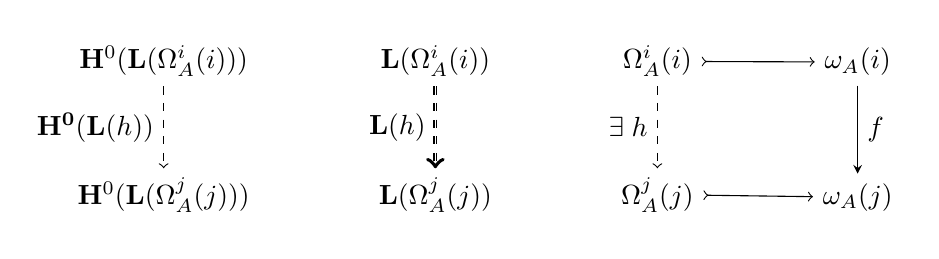
\begin{tikzpicture}
	\matrix (m) [matrix of math nodes,row sep=3em,column sep=4em,minimum width=2em]
	{
		\mathbf{H}^0(\mathbf{L}( \Omega^i_A(i) )) & \mathbf{L}( \Omega^i_A(i) ) & \Omega^i_A(i) & \omega_A(i) \\
		\mathbf{H}^0(\mathbf{L}( \Omega^j_A(j) )) & \mathbf{L}( \Omega^j_A(j) ) & \Omega^j_A(j) & \omega_A(j) \\};
	\path[-stealth]
	
	(m-1-1) edge [dashed,->] node [left] {$\mathbf{H^0(L}(h))$} (m-2-1)
	(m-1-2) edge [double,dashed,->] node [left] {$\mathbf{L}(h)$} (m-2-2)
	(m-1-3) edge [dashed,->] node [left] {$\exists\;h$} (m-2-3)
		edge [>->] (m-1-4)
	(m-2-3.east|-m-2-2) edge [>->] (m-2-4)
	(m-1-4) edge node [right] {$f$} (m-2-4);
  \end{tikzpicture}
\]

Let $U:A\mbox{-gmod} \rightarrow A\mbox{-gmod}$ be the endomorphism defined by
$U(\omega_A(i)\rightarrow \omega_A(j))=\Omega_A^i(i)\rightarrow \Omega_A^i(j).$
\begin{Verbatim}[commandchars=\\\{\}]
\textcolor{red}{w_2 := w_A(2);}
<An object in The category of graded left f.p. modules over Q\{e0,e1,e2,e3\} (with weights [ -1, -1, -1, -1 ])>
\textcolor{red}{w_0 := w_A(0);}
<An object in The category of graded left f.p. modules over Q\{e0,e1,e2,e3\} (with weights [ -1, -1, -1, -1 ])>
\textcolor{red}{Display( w_2 );}
(an empty 0 x 1 matrix)

An object in The category of graded left f.p. modules over Q\{e0,e1,e2,e3\} (with weights [ -1, -1, -1, -1 ])

(graded, degree of generator:[ 2 ])
\textcolor{red}{Display( w_0 );}
(an empty 0 x 1 matrix)

An object in The category of graded left f.p. modules over Q\{e0,e1,e2,e3\} (with weights [ -1, -1, -1, -1 ])

(graded, degree of generator:[ 4 ])
\textcolor{red}{g := graded_generators_of_external_hom(w_2,w_0);;}
\textcolor{red}{f := Sum(g);}
<A morphism in The category of graded left f.p. modules over Q\{e0,e1,e2,e3\} (with weights [ -1, -1, -1, -1 ])>
\textcolor{red}{Display(f);}
-e0*e1-e0*e2-e1*e2-e0*e3-e1*e3-e2*e3
(over a graded ring)
	
A morphism in The category of graded left f.p. modules over Q\{e0,e1,e2,e3\} (with weights [ -1, -1, -1, -1 ])
\textcolor{red}{U := ToMorphismBetweenCotangentBundlesFunctor;;}
\textcolor{red}{h := ApplyFunctor( U, f );}
<A morphism in The category of graded left f.p. modules over Q\{e0,e1,e2,e3\} (with weights [ -1, -1, -1, -1 ])>
\textcolor{red}{Display(h);}
1, 
-1,
1, 
1, 
-1,
1  
(over a graded ring)
	
A morphism in The category of graded left f.p. modules over Q\{e0,e1,e2,e3\} (with weights [ -1, -1, -1, -1 ])
\textcolor{red}{IsWellDefined( h );}
true
\textcolor{red}{Lh := ApplyFunctor( L, h );}
<A bounded morphism in cochain complexes category over the category of graded left f.p. modules over 
Q[x0,x1,x2,x3] (with weights [ 1, 1, 1, 1 ]) with active lower bound -1 and active upper bound 5>
\textcolor{red}{H0 := CohomologyFunctorAt( cochains_graded_lp_cat_sym, graded_lp_cat_sym, 0 );}
0-th cohomology functor in the category of graded left f.p. modules over Q[x0,x1,x2,x3] 
(with weights [ 1, 1, 1, 1 ])
\textcolor{red}{H0_Lh := ApplyFunctor( H0, Lh );}
<A morphism in The category of graded left f.p. modules over Q[x0,x1,x2,x3] (with weights [ 1, 1, 1, 1 ])>
\textcolor{red}{Display( Source( H0_Lh ) );}
x0,-x3,-x2,-x1
(over a graded ring)
	
An object in The category of graded left f.p. modules over Q[x0,x1,x2,x3] (with weights [ 1, 1, 1, 1 ])
	
(graded, degrees of generators:[ 1, 1, 1, 1 ])
\textcolor{red}{Display( omega_S_2_2 );}
-x0,x1,x3,-x2
(over a graded ring)
	
An object in The category of graded left f.p. modules
over Q[x0,x1,x2,x3] (with weights [ 1, 1, 1, 1 ])
	
(graded, degrees of generators:[ 1, 1, 1, 1 ])
\textcolor{red}{Display( Range( H0_Lh ) );}
(an empty 0 x 1 matrix)
	
An object in The category of graded left f.p. modules over Q[x0,x1,x2,x3] (with weights [ 1, 1, 1, 1 ])
	
(graded, degree of generator:[ 0 ])
\textcolor{red}{Display( omega_S_0 );}
0, 0,  x3, -x2,
0, x2, -x1,0,  
0, x3, 0,  -x1,
x1,-x0,0,  0,  
x2,0,  -x0,0,  
x3,0,  0,  -x0 
(over a graded ring)

An object in The category of graded left f.p. modules
over Q[x0,x1,x2,x3] (with weights [ 1, 1, 1, 1 ])

(graded, degrees of generators:[ 1, 1, 1, 1 ])
\end{Verbatim}

\section{Beilinson Monad}
Let us now compute the Beilinson Monad of a coherent sheaf given by the sheafification of graded f.p. $S$-module.

\begin{Verbatim}[commandchars=\\\{\}]
\textcolor{red}{m := RandomMatrixBetweenGradedFreeLeftModules([2,1],[1,-1,2],S);}
<A 2 x 3 matrix over a graded ring>
\textcolor{red}{M := AsGradedLeftPresentation(m,[1,-1,2]);}
<An object in The category of graded left f.p. modules over Q[x0,x1,x2,x3] (with weights [ 1, 1, 1, 1 ])>
\textcolor{red}{Display( M );}
-2*x0+2*x1+4*x2,_[1,2],                                          -2,
-1,             2*x0*x1+x0*x2-2*x1*x2-5*x2^2-x0*x3-4*x1*x3-x2*x3,0  
(over a graded ring)

An object in The category of graded left f.p. modules over Q[x0,x1,x2,x3] (with weights [ 1, 1, 1, 1 ])

(graded, degrees of generators:[ 1, -1, 2 ])
\textcolor{red}{Tate := TateFunctor( S );}
Tate 'functor' from The category of graded left f.p. modules over Q[x0,x1,x2,x3] 
(with weights [ 1, 1, 1, 1 ]) to Cochain complexes category over the category of graded left f.p. modules 
over Q\{e0,e1,e2,e3\} (with weights [ -1, -1, -1, -1 ])
\textcolor{red}{TM := ApplyFunctor( Tate, M );;}
\textcolor{red}{U := ToMorphismBetweenCotangentBundlesFunctor;;}
\textcolor{red}{ChU := ExtendFunctorToCochainComplexCategories(U);;}
\textcolor{red}{ChU_TM := ApplyFunctor( ChU, TM );;}
\textcolor{red}{L := LFunctor( S );}
L functor from The category of graded left f.p. modules over Q\{e0,e1,e2,e3\} 
(with weights [ -1, -1, -1, -1 ]) to Cochain complexes category over the category of 
graded left f.p. modules over Q[x0,x1,x2,x3] (with weights [ 1, 1, 1, 1 ])
\textcolor{red}{ChL := ExtendFunctorToCochainComplexCategories(L);;}
\textcolor{red}{ChL_ChU_TM := ApplyFunctor( ChL, ChU_TM );;}
\textcolor{red}{B := CohomologicalBicomplex( ChL_ChU_TM );}
<A cohomological bicomplex in The category of graded left f.p. modules over Q[x0,x1,x2,x3] 
(with weights [ 1, 1, 1, 1 ]) concentrated in window 
[ -inf.. inf ] x [ -inf .. inf ]>
\textcolor{red}{SupportInWindow( B, -4, 4, -4, 4 );}
. . . . . . . . .   |4
. . . . . . . . .   |3
. . . . . . . . .   |2
. . . * . . . . .   |1
. . . * * . . . .   |0
. . . . . . . . .   |-1
. . . . . . . . .   |-2
. . . . . . . . .   |-3
. . . . . . . . .   |-4
\textcolor{red}{SetRight_Bound( B, 1 );;}
\textcolor{red}{SetLeft_Bound( B, -2 );;}
\textcolor{red}{T := TotalComplex( B );}
<An object in Cochain complexes category over the category of graded left f.p. modules over Q[x0,x1,x2,x3] 
(with weights [ 1, 1, 1, 1 ])>
\textcolor{red}{CohomologySupport( T, -4, 4 );}
[ 0 ]
\textcolor{red}{H0 := CohomologyFunctorAt( cochains_graded_lp_cat_sym, graded_lp_cat_sym, 0 );}
0-th cohomology functor in the category of graded left f.p. modules over Q[x0,x1,x2,x3] 
(with weights [ 1, 1, 1, 1 ])
\textcolor{red}{H0_T := ApplyFunctor( H0, T );}
<An object in The category of graded left f.p. modules over Q[x0,x1,x2,x3] (with weights [ 1, 1, 1, 1 ])>
\textcolor{red}{Display( H0_T );}
2,0,0, 0, x0, 
0,2,-1,-1,-x1,
0,4,0, 0, x2, 
0,0,-2,0, -x3 
(over a graded ring)

An object in The category of graded left f.p. modules over Q[x0,x1,x2,x3] (with weights [ 1, 1, 1, 1 ])

(graded, degrees of generators:[ 0, 0, 0, 0, -1 ])
\textcolor{red}{Display( M );}
-2*x0+2*x1+4*x2,_[1,2],                                          -2,
-1,             2*x0*x1+x0*x2-2*x1*x2-5*x2^2-x0*x3-4*x1*x3-x2*x3,0  
(over a graded ring)

An object in The category of graded left f.p. modules over Q[x0,x1,x2,x3] (with weights [ 1, 1, 1, 1 ])

(graded, degrees of generators:[ 1, -1, 2 ])
\textcolor{red}{syz0_M := Source( CyclesAt( ApplyFunctor( Tate, M ), 0 ) );}
<An object in The category of graded left f.p. modules over Q\{e0,e1,e2,e3\} (with weights [ -1, -1, -1, -1 ])>
\textcolor{red}{syz0_H0_T := Source( CyclesAt( ApplyFunctor( Tate, H0_T ), 0 ) );}
<An object in The category of graded left f.p. modules over Q\{e0,e1,e2,e3\} (with weights [ -1, -1, -1, -1 ])>
\textcolor{red}{Display( syz0_M );}
e0*e1*e2*e3
(over a graded ring)

An object in The category of graded left f.p. modules over Q\{e0,e1,e2,e3\} (with weights [ -1, -1, -1, -1 ])

(graded, degree of generator:[ 3 ])
\textcolor{red}{Display( syz0_H0_T );}
e0*e1*e2*e3
(over a graded ring)

An object in The category of graded left f.p. modules over Q\{e0,e1,e2,e3\} (with weights [ -1, -1, -1, -1 ])

(graded, degree of generator:[ 3 ])
\end{Verbatim}
\end{document}